\documentclass{standalone}
\usepackage{tikz}
\usetikzlibrary{patterns, positioning}


\begin{document}
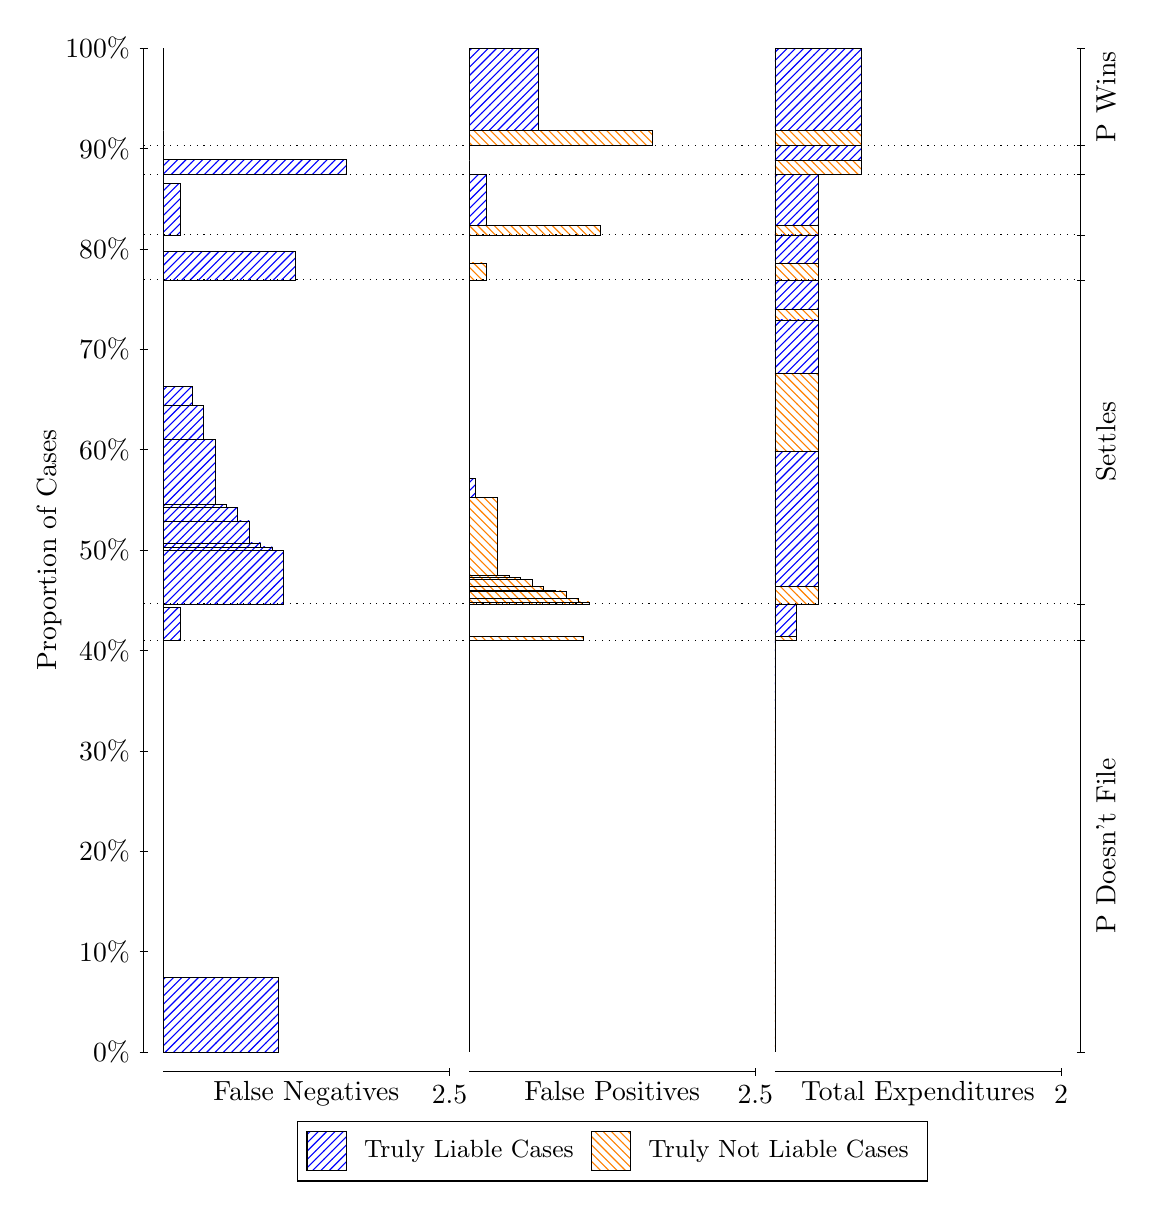
\begin{tikzpicture}
\draw[black, very thin] (1.5,1.75) -- (1.5,14.5);
\node[rotate=90, text=black, anchor=center] at (0.3, 8.125) {Proportion of Cases};
\draw[black, very thin] (1.45,1.75) -- (1.55,1.75);
\node[text=black, anchor=east] at (1.45, 1.75) {0\%};
\draw[black, very thin] (1.45,3.025) -- (1.55,3.025);
\node[text=black, anchor=east] at (1.45, 3.025) {10\%};
\draw[black, very thin] (1.45,4.3) -- (1.55,4.3);
\node[text=black, anchor=east] at (1.45, 4.3) {20\%};
\draw[black, very thin] (1.45,5.575) -- (1.55,5.575);
\node[text=black, anchor=east] at (1.45, 5.575) {30\%};
\draw[black, very thin] (1.45,6.85) -- (1.55,6.85);
\node[text=black, anchor=east] at (1.45, 6.85) {40\%};
\draw[black, very thin] (1.45,8.125) -- (1.55,8.125);
\node[text=black, anchor=east] at (1.45, 8.125) {50\%};
\draw[black, very thin] (1.45,9.4) -- (1.55,9.4);
\node[text=black, anchor=east] at (1.45, 9.4) {60\%};
\draw[black, very thin] (1.45,10.675) -- (1.55,10.675);
\node[text=black, anchor=east] at (1.45, 10.675) {70\%};
\draw[black, very thin] (1.45,11.95) -- (1.55,11.95);
\node[text=black, anchor=east] at (1.45, 11.95) {80\%};
\draw[black, very thin] (1.45,13.225) -- (1.55,13.225);
\node[text=black, anchor=east] at (1.45, 13.225) {90\%};
\draw[black, very thin] (1.45,14.5) -- (1.55,14.5);
\node[text=black, anchor=east] at (1.45, 14.5) {100\%};

\draw[black, very thin] (13.4,1.75) -- (13.4,14.5);
\draw[black, very thin] (13.35,1.75) -- (13.45,1.75);
\node[anchor=west] at (13.35, 1.75) {};
\draw[black, very thin] (13.35,6.9807) -- (13.45,6.9807);
\node[anchor=west] at (13.35, 6.9807) {};
\draw[black, very thin] (13.35,7.4416) -- (13.45,7.4416);
\node[anchor=west] at (13.35, 7.4416) {};
\draw[black, very thin] (13.35,11.556) -- (13.45,11.556);
\node[anchor=west] at (13.35, 11.556) {};
\draw[black, very thin] (13.35,12.128) -- (13.45,12.128);
\node[anchor=west] at (13.35, 12.128) {};
\draw[black, very thin] (13.35,12.897) -- (13.45,12.897);
\node[anchor=west] at (13.35, 12.897) {};
\draw[black, very thin] (13.35,13.261) -- (13.45,13.261);
\node[anchor=west] at (13.35, 13.261) {};
\draw[black, very thin] (13.35,14.5) -- (13.45,14.5);
\node[anchor=west] at (13.35, 14.5) {};

\draw[black, very thin, pattern color=blue, pattern=north east lines] (1.75,1.75) rectangle (3.2033,2.6996);
\draw[black, very thin, pattern color=orange, pattern=north west lines] (1.75,2.6996) rectangle (1.75,6.9807);
\draw[black, very thin, pattern color=blue, pattern=north east lines] (1.75,6.9807) rectangle (1.968,7.3988);
\draw[black, very thin, pattern color=orange, pattern=north west lines] (1.75,7.3988) rectangle (1.75,7.4416);
\draw[black, very thin, pattern color=blue, pattern=north east lines] (1.75,7.4416) rectangle (3.276,8.118);
\draw[black, very thin, pattern color=blue, pattern=north east lines] (1.75,8.118) rectangle (3.1307,8.1633);
\draw[black, very thin, pattern color=blue, pattern=north east lines] (1.75,8.1633) rectangle (2.9853,8.2146);
\draw[black, very thin, pattern color=blue, pattern=north east lines] (1.75,8.2146) rectangle (2.84,8.4939);
\draw[black, very thin, pattern color=blue, pattern=north east lines] (1.75,8.4939) rectangle (2.6947,8.6625);
\draw[black, very thin, pattern color=blue, pattern=north east lines] (1.75,8.6625) rectangle (2.5493,8.7088);
\draw[black, very thin, pattern color=blue, pattern=north east lines] (1.75,8.7088) rectangle (2.404,9.5337);
\draw[black, very thin, pattern color=blue, pattern=north east lines] (1.75,9.5337) rectangle (2.2587,9.9598);
\draw[black, very thin, pattern color=blue, pattern=north east lines] (1.75,9.9598) rectangle (2.1133,10.205);
\draw[black, very thin, pattern color=orange, pattern=north west lines] (1.75,10.205) rectangle (1.75,11.556);
\draw[black, very thin, pattern color=blue, pattern=north east lines] (1.75,11.556) rectangle (3.4213,11.913);
\draw[black, very thin, pattern color=orange, pattern=north west lines] (1.75,11.913) rectangle (1.75,12.128);
\draw[black, very thin, pattern color=blue, pattern=north east lines] (1.75,12.128) rectangle (1.968,12.78);
\draw[black, very thin, pattern color=orange, pattern=north west lines] (1.75,12.78) rectangle (1.75,12.897);
\draw[black, very thin, pattern color=blue, pattern=north east lines] (1.75,12.897) rectangle (4.0753,13.086);
\draw[black, very thin, pattern color=orange, pattern=north west lines] (1.75,13.086) rectangle (1.75,13.261);
\draw[black, very thin, pattern color=orange, pattern=north west lines] (1.75,13.261) rectangle (1.75,13.454);
\draw[black, very thin, pattern color=blue, pattern=north east lines] (1.75,13.454) rectangle (1.75,14.5);
\draw[black, very thin, pattern color=orange, pattern=north west lines] (5.6333,1.75) rectangle (5.6333,6.0311);
\draw[black, very thin, pattern color=blue, pattern=north east lines] (5.6333,6.0311) rectangle (5.6333,6.9807);
\draw[black, very thin, pattern color=orange, pattern=north west lines] (5.6333,6.9807) rectangle (7.0867,7.0235);
\draw[black, very thin, pattern color=blue, pattern=north east lines] (5.6333,7.0235) rectangle (5.6333,7.4416);
\draw[black, very thin, pattern color=orange, pattern=north west lines] (5.6333,7.4416) rectangle (7.1593,7.4666);
\draw[black, very thin, pattern color=orange, pattern=north west lines] (5.6333,7.4666) rectangle (7.014,7.5112);
\draw[black, very thin, pattern color=orange, pattern=north west lines] (5.6333,7.5112) rectangle (6.8687,7.6068);
\draw[black, very thin, pattern color=orange, pattern=north west lines] (5.6333,7.6068) rectangle (6.7233,7.6141);
\draw[black, very thin, pattern color=orange, pattern=north west lines] (5.6333,7.6141) rectangle (6.578,7.6598);
\draw[black, very thin, pattern color=orange, pattern=north west lines] (5.6333,7.6598) rectangle (6.4327,7.6608);
\draw[black, very thin, pattern color=orange, pattern=north west lines] (5.6333,7.6608) rectangle (6.4327,7.7505);
\draw[black, very thin, pattern color=orange, pattern=north west lines] (5.6333,7.7505) rectangle (6.2873,7.7752);
\draw[black, very thin, pattern color=orange, pattern=north west lines] (5.6333,7.7752) rectangle (6.142,7.7979);
\draw[black, very thin, pattern color=orange, pattern=north west lines] (5.6333,7.7979) rectangle (5.9967,8.793);
\draw[black, very thin, pattern color=blue, pattern=north east lines] (5.6333,8.793) rectangle (5.706,9.038);
\draw[black, very thin, pattern color=blue, pattern=north east lines] (5.6333,9.038) rectangle (5.6333,11.556);
\draw[black, very thin, pattern color=orange, pattern=north west lines] (5.6333,11.556) rectangle (5.8513,11.77);
\draw[black, very thin, pattern color=blue, pattern=north east lines] (5.6333,11.77) rectangle (5.6333,12.128);
\draw[black, very thin, pattern color=orange, pattern=north west lines] (5.6333,12.128) rectangle (7.3047,12.245);
\draw[black, very thin, pattern color=blue, pattern=north east lines] (5.6333,12.245) rectangle (5.8513,12.897);
\draw[black, very thin, pattern color=orange, pattern=north west lines] (5.6333,12.897) rectangle (5.6333,13.072);
\draw[black, very thin, pattern color=blue, pattern=north east lines] (5.6333,13.072) rectangle (5.6333,13.261);
\draw[black, very thin, pattern color=orange, pattern=north west lines] (5.6333,13.261) rectangle (7.9587,13.454);
\draw[black, very thin, pattern color=blue, pattern=north east lines] (5.6333,13.454) rectangle (6.5053,14.5);
\draw[black, very thin, pattern color=orange, pattern=north west lines] (9.5167,1.75) rectangle (9.5167,6.0311);
\draw[black, very thin, pattern color=blue, pattern=north east lines] (9.5167,6.0311) rectangle (9.5167,6.9807);
\draw[black, very thin, pattern color=orange, pattern=north west lines] (9.5167,6.9807) rectangle (9.7892,7.0235);
\draw[black, very thin, pattern color=blue, pattern=north east lines] (9.5167,7.0235) rectangle (9.7892,7.4416);
\draw[black, very thin, pattern color=orange, pattern=north west lines] (9.5167,7.4416) rectangle (10.062,7.6608);
\draw[black, very thin, pattern color=blue, pattern=north east lines] (9.5167,7.6608) rectangle (10.062,9.3758);
\draw[black, very thin, pattern color=orange, pattern=north west lines] (9.5167,9.3758) rectangle (10.062,10.371);
\draw[black, very thin, pattern color=blue, pattern=north east lines] (9.5167,10.371) rectangle (10.062,11.047);
\draw[black, very thin, pattern color=orange, pattern=north west lines] (9.5167,11.047) rectangle (10.062,11.184);
\draw[black, very thin, pattern color=blue, pattern=north east lines] (9.5167,11.184) rectangle (10.062,11.556);
\draw[black, very thin, pattern color=orange, pattern=north west lines] (9.5167,11.556) rectangle (10.062,11.77);
\draw[black, very thin, pattern color=blue, pattern=north east lines] (9.5167,11.77) rectangle (10.062,12.128);
\draw[black, very thin, pattern color=orange, pattern=north west lines] (9.5167,12.128) rectangle (10.062,12.245);
\draw[black, very thin, pattern color=blue, pattern=north east lines] (9.5167,12.245) rectangle (10.062,12.897);
\draw[black, very thin, pattern color=orange, pattern=north west lines] (9.5167,12.897) rectangle (10.607,13.072);
\draw[black, very thin, pattern color=blue, pattern=north east lines] (9.5167,13.072) rectangle (10.607,13.261);
\draw[black, very thin, pattern color=orange, pattern=north west lines] (9.5167,13.261) rectangle (10.607,13.454);
\draw[black, very thin, pattern color=blue, pattern=north east lines] (9.5167,13.454) rectangle (10.607,14.5);
\draw[black, dotted] (1.5,6.9807) -- (13.4,6.9807);
\draw[black, dotted] (1.5,7.4416) -- (13.4,7.4416);
\draw[black, dotted] (1.5,11.556) -- (13.4,11.556);
\draw[black, dotted] (1.5,12.128) -- (13.4,12.128);
\draw[black, dotted] (1.5,12.897) -- (13.4,12.897);
\draw[black, dotted] (1.5,13.261) -- (13.4,13.261);
\draw[black, very thin] (1.75,1.5) -- (5.3833,1.5);
\node[text=black, anchor=north] at (3.5667, 1.5) {False Negatives};
\draw[black, very thin] (5.3833,1.45) -- (5.3833,1.55);
\node[text=black, anchor=north] at (5.3833, 1.45) {2.5};

\draw[black, very thin] (5.6333,1.5) -- (9.2667,1.5);
\node[text=black, anchor=north] at (7.45, 1.5) {False Positives};
\draw[black, very thin] (9.2667,1.45) -- (9.2667,1.55);
\node[text=black, anchor=north] at (9.2667, 1.45) {2.5};

\draw[black, very thin] (9.5167,1.5) -- (13.15,1.5);
\node[text=black, anchor=north] at (11.333, 1.5) {Total Expenditures};
\draw[black, very thin] (13.15,1.45) -- (13.15,1.55);
\node[text=black, anchor=north] at (13.15, 1.45) {2};

\node[text=black, centered, rotate=90] at (13.72, 4.3653) {P Doesn't File};

\node[text=black, centered, rotate=90] at (13.72, 9.4989) {Settles};



\node[text=black, centered, rotate=90] at (13.72, 13.881) {P Wins};

\draw (7.449999999999999,1.5) node[draw=none] (baseCoordinate) {};
\begin{scope}[align=center]
        \matrix[scale=0.5, draw=black, below=0.5cm of baseCoordinate, nodes={draw}, column sep=0.1cm]{
            \node[rectangle, draw, minimum width=0.5cm, minimum height=0.5cm, pattern color=blue, pattern=north east lines] {}; &
            \node[draw=none, font=\small, text=black] (B) {Truly Liable Cases}; &
            \node[rectangle, draw, minimum width=0.5cm, minimum height=0.5cm, pattern color=orange, pattern=north west lines] {}; &
            \node[draw=none, font=\small, text=black] (B) {Truly Not Liable Cases}; \\
            };
\end{scope}

\end{tikzpicture}
\end{document}